\section{Introduction}\label{sec:introduction}

In the Western music canon, 
%(and especially in popular music), 
\emph{melody} is a defining characteristic of musical composition. 
Even those without formal musical training can often effortlessly recognize a melody within a complex mixture of sounds, 
a ubiquitous skill which forms a pillar of our collective musical experience. %experience. 
Because of the significance of melody to music perception, 
the ability to automatically \emph{transcribe} the melody notes present in an arbitrary recording 
could enable numerous applications in 
% TODO: performance?
interaction~\cite{ryynanen2008accompaniment}, 
education~\cite{droe2006music}, 
informatics~\cite{bainbridge1999towards}, 
retrieval~\cite{ghias1995query}, 
source separation~\cite{ewert2014score},
and even generation~\cite{hawthorne2019enabling}.
Despite the potential benefits, 
reliable melody transcription remains an open challenge in MIR.

The relative lack of progress on melody transcription is perhaps counterintuitive when compared to the considerable progress on seemingly more difficult tasks like piano transcription~\cite{sigtia2016end,hawthorne2017onsets}.
%and chord recognition~\cite{humphrey2012rethinking,boulanger2013audio}. 
This circumstance stems from two primary factors. 
First, unlike in piano transcription, melody transcription involves operating on \emph{broad}
% CHRIS: I like broad slightly more I think
%\john{diverse?} 
audio mixtures from arbitrary instrument ensembles and genres. 
% CHRIS: I think the following are indeed reasons that melody transcription is hard, but they don't map as cleanly onto our contributions
%Second, unlike in chord recognition, melody transcription involves isolating the notes from a single instrument voice (recognized to be the melodic voice) within the mixture. 
%Second, melody transcription involves not only detecting notes but also identifying which of those notes constitutes the melody, which may require modeling the nuances of human music perception. 
Second, little training data exists for melody transcription, which particularly impedes the deep learning approaches central to recent improvements in other transcription settings. 

\begin{figure}
    \centering
    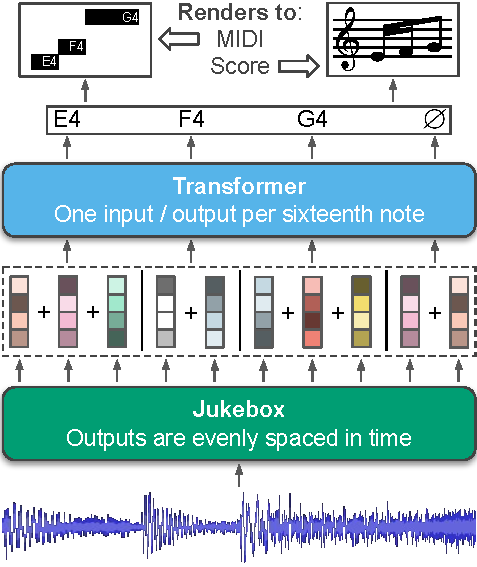
\includegraphics[width=8.1cm]{figs/fig1.pdf}
    \caption{
Our melody transcription approach involves 
(1)~extracting audio representations from Jukebox~\cite{dhariwal2020jukebox}, a generative model of music, 
(2)~averaging these representations across time to their nearest sixteenth note (dashed outline---uses \madmom{}~\cite{bock2016joint,bock2016madmom} for beat detection),
and
(3)~training a Transformer~\cite{vaswani2017attention} to detect melody note onsets (or absence thereof) per sixteenth note. 
}
 \label{fig:fig1}
\end{figure}

To overcome the challenge of transcribing broad audio, in this work we leverage representations from Jukebox~\cite{dhariwal2020jukebox}, a large-scale generative model of music audio pre-trained on $1$M songs~(\Cref{fig:fig1}). 
In~\cite{castellon2021calm}, Castellon~et~al.\ demonstrate that internal representations from Jukebox are useful for improving performance on a wide variety of MIR tasks. 
When used as input features to a Transformer model~\cite{vaswani2017attention}, representations from Jukebox outperform conventional spectrogram features used for melody transcription by 
% (RWC All) .744 vs .631 = 17.9%
% (Hookthr) .615 vs .514 = 19.6%
% (RWC Vox) .786 vs .621 = 26.6%
up to $27$\% (relative). 
% CHRIS: This was written conservatively because but could potentially be broadened... this may be the first time transfer learning has ever been used for transcription or any time-varying MIR task (though MT3 may be one instance)
To the best of our knowledge, this is the first evidence that representations learned through generative modeling are useful for time-varying MIR tasks like transcription, as opposed to the song-level tasks (e.g.~tagging, genre detection) examined in~\cite{castellon2021calm}.

\john{Weak topic sentence. And this paragraph is kind of all over the place}
To support this and future work on melody transcription, we collect and release a new dataset of crowdsourced melody annotations from the \hooktheory{} platform.\footnote{\url{https://www.hooktheory.com/theorytab}} 
This dataset contains $50$ hours of annotated melodies and harmonies (as chord names) aligned with audio recordings available on YouTube. 
%to aid chord recognition research. 
By training Transformer models on this new dataset using representations from Jukebox, we are able to improve overall performance on melody transcription by 
% 0.786 vs 0.462 = 70%
% 0.744 vs 0.420 = 77%
up to $77$\% 
relative to the strongest available baseline. 
We also release all code and models needed to precisely reproduce all of our evaluations,\footnote{Released upon publication} facilitating comparison in future work even as some audio inevitably disappears from YouTube.

\john{Maybe too many details? Content of this and previous paragraph might benefit from reorg/streamlining}
We also propose a new method for training transcription models in the presence of imprecise audio-to-score alignments. 
% Existing transcription methods were largely designed for domains where perfect alignments are readily available, e.g.,~a Disklavier yields piano transcription data with perfect alignment. 
% The alignments in \hooktheory{} are not precise enough to facilitate effective transcription when adopting these methods off-the-shelf. 
% To address this, we propose a new method which  
Our approach 
involves aggregating input features (evenly spaced in \emph{time}) into proxy features representative of individual sixteenth notes (evenly spaced in \emph{beats}), 
thereby smoothing over alignment jitter. 
We train models on these beat-based features, 
which has a secondary benefit of enabling simple conversion from raw model outputs to human-readable scores (\Cref{fig:fig1}).

%\textbf{Contributions.} 
A summary of our primary \textbf{contributions} is as follows:
\begin{itemize}
    \item We show that representations from generative models can improve melody transcription (\Cref{sec:experiments}).
    \item We collect, align, and release a new dataset with $50$ hours of melody and chord annotations (\Cref{sec:dataset}).
    \item We propose a method for training transcription models on data with imprecise alignment (\Cref{sec:beatpool}).
    \item As a downstream application of our melody transcription approach, we build a system which can transcribe music audio into lead sheets (\Cref{sec:sheetsage}).
\end{itemize}